\documentclass{article}
\usepackage{amsmath}
\usepackage{amsfonts}
\usepackage{mathtools}
\usepackage[ruled]{algorithm2e}
\usepackage{graphicx}
\graphicspath{ {./images/} }

\title{Regression Tree Learning \\ 
    \large Costruzione, pruning e metodi ensemble}
\author{Ivan Diliso Matricola: 676366 \\
Email: \textit{diliso.ivan@gmail.com} \\
    Progetto di Ingegneria della Conoscenza}
\date{}

\begin{document}
    \maketitle

    \newpage

    \tableofcontents{}

    \newpage

    \section{Introduzione}
    \paragraph{Apprendimento supervisionato}
    Il problema dell'apprendimento supervisionato richiede
    che si apprenda una funzione a partire da esempi di input e output.
    Dato un insieme di esempi \((x, f(x))\) con \(x\) input e \(f(x)\)
    l'output della funzione applicata a \(x\), il compito dell'apprendimento
    supervisionato è restituire una funzone \(h\) che approssima \(f\). \\

    L'apprendimento tramite alberi di regressione è una forma di apprendimento
    supervisionato che permette l'approssimazione di funzioni a valori continui
    a partire da un insieme di esempi chiamato insieme di training. Un albero di
    regressione funziona eseguendo una serie di test, ogni nodo interno dell'albero
    corrisponde ad un test sul valore di una delle feature dell'insieme di training
    e le diramazioni uscenti sono etichettate con tutti i possibili risultati. I nodi 
    foglia specificano il valore da fornire in uscita. 
    Questo progetto descrive l'implementazione di tutte le fasi che portano alla costruzione di un albero 
    di regressione, quali: preprocessing dei dati, ricerca della feature di split e del
    treshold ottimale per lo split e valutazione.
    Vengono inoltre descritti un metodo per il pruning di alberi molto grandi (Cost 
    complexity pruning) e metodi di apprendimento ensemble per alberi di regressione
    (Bagging e Random Forest). Verranno inoltre confrontate le varie metodologie 
    implementate.
    (Regression Tree, Pruned Regression Tree, Bagging e Random Forest)


    \section{Preprocessing}
    Il sistema implementato non è in grado di gestire feature a valori non continui 
    o con dati mancanti. Nella fase di preprocessing il dataset viene modificato in 
    modo da aderire agli standard del sistema. Il problema dei dati mancanti è stato
    risolto eliminando dal dataset ogni esempio contente una o più feature con valori
    non presenti. Verranno inoltre rimosse dal dataset tutte le feature che presentano
    una sola modalità. 

    \paragraph{Dataset}

    Insieme degli esempi $(x_i, y_i)$ per $ i=1,2,\ldots,N$ con \\
    $ x_i = (x_{i1},x_{i2},\ldots,x_{ik})$
    e $k$ numero di feature di input del dataset.

    \subsection{Feature dicotomiche}
    Una feature dicotomica è una feature che presenta soltanto due modalità. Sono dicotomiche
    feature con valori come \{si, no\}, oppure \{vero, falso\}. In questo caso verranno 
    assegnati i valori \{0,1\} rispettivamente alle due modalità, in ogni esempio verrà sostituito
    il valore iniziale della modalità con il nuovo valore assegnato.

    \subsection{Feature categoriche}
    Una feature categorica è una feature che presenta più di due modalità. In questo caso 
    viene utilizzata una tecnica di encoding chiamata "One-Hot". 
    Sia \(n\) il numero di esempi nel dataset, sia \(f\) ( con \(k > 2\) modalità
    diverse $\{v_1, v_2, \cdots ,v_k\}$) la feature da codificare e sia $f(x_i)$ il valore di $f$ 
    per l'i-esimo esempio del dataset.
    Il metodo one-hot produrrà \(k\) nuove feature
    $\{f_1, f_2, \cdots ,f_k\}$
    tali che per ogni feature (con $ 1 <= j <= k$):
    
    \[
        f_j(x_i)=
        \begin{cases}
            1, & \text{if } f(x_i)=v_j \\
            0, & \text{otherwise}
        \end{cases}
    \]

    Una feature categorica a k valori verrà quindi trasformata in k feature binarie.
    La feature categorica originale verrà rimossa dal dataset
    

    \section{Alberi di regressione}
    La principale problematica
    nella costruzione di un albero di regressione è la scelta della feature e treshold 
    di split in grado di creare partizioni del dataset che 
    minimizzano una metrica definita.


    Definiamo quindi prima come viene costruito l'albero per poi passare ai dettagli 
    della scelta del valore di split.


    \subsection{Recursive binary splitting}
    Seguendo la metodologia
    \textit{CART} l'albero viene costruito tramite 
    \textit{recursive binary splitting}. Ogni test dividerà il training set in due 
    partizioni, scelta la feature di split $f_j$ 
    e il valore di split $v_j$ ($min(f_j) <= v <= max(f_j)$) il test avrà forma 
    $ f_j(i) < v_j$. La procedura verrà quindi ripetuta sulle nuove partizioni ottenute
    (la partizione di sinistra rappresenta il nodo figlio sinistro 
    contentente gli esempi  $\{x_i | f_j(x_i) < v_j\}$, la partizione descritta
    il nodo figlio destro contentente gli esempi  $\{x_i | f_j(x_i) >= v_j\}$)
    Questa procedura verrà ripetuta finchè il numero di esempi in una partizione non sarà 
    minore o uguale di un parametro di tuning \textit{leaf\_size}. 

    \subsection{Criterio di split}
    Data una partizione del dataset in $M$ regioni $R_1,R_2,\ldots,R_M$, definiamo 
    la predizione di ogni partizione ($c_m$) come la media dei valori della feature target 
    $y_i$ presenti all'interno della partizione

    \[
        c_m = ave(y_i|x_i \in R_m)  
    \]

    La feature e il relativo valore di split verranno scelti in base
    ad un criterio di minimizzazione dell'errore su tutte le partizioni.
    Per task di regressione una delle metriche consigliate è la \textit{residual sum of squares}

    \[
        \text{SSR}= \sum_{} (y_i - f(x_i))^2
    \]

    In questo caso avendo scelto il \textit{recursive binary splitting} le partizioni
    saranno soltanto due, $R_l$ e $R_r$. Scelta quindi la feature $f_j$
    e il valore $v_j$ le due partizioni saranno rispettivamente:

    \[
        R_l(f_j, v_j) = \{x_i | f_j(x_i) < v_j\}  \text{  e  } R_r(f_j, v_j) = \{x_i | f_j(x_i) >= v_j\}
    \]

    Per la scelta dei valori di split $f_j$ e $v_j$ verrà utilizzato un approccio
    greedy che andrà a scegliere i valori $f_j$ e $v_j$ che risolvono:

    \[
        \min_{f_j, v_j} \left[ 
        \min_{c_l} 
        \sum_{x_i \in R_l(f_j, v_j)} (y_i - c_l)^2 + 
        \min_{c_r} 
        \sum_{x_i \in R_r(f_j, v_j)} (y_i - c_r)^2
        \right]
    \]

    con
     \[
         c_l = ave(y_i| x_i \in R_l) \text{ e  }  c_r = ave(y_i| x_i \in R_r)
     \]

     \subsection{Valori di split}
     Data una feature $f_j$ definiamo l'insieme $V_{f_j}=\{v_1,v_2,\ldots,v_l\}$ 
     tale che $\forall v_h,v_k \in V_{f_j}  \text{ }1 \leq h,k \leq l \text{ }
     \text{ se } h < k \text{ allora } v_h < v_k$ cioè l'insieme degli elementi dei
     valori della feature $f_j$ presi una ed una sola volta e ordinati in ordine crescente.
     L'insieme dei varoli della feature che verranno considerati per la ricerca 
     della miglior treshold saranno:
        
        \[
          VS_{f_j} = \{v | v=\frac{(v_h + v_{h+1})}{2} \text{ con } 1 \leq h \leq l-1\}  
        \]
        
        
    \subsection{Parametri di tuning}
    Nella creazione di un albero di regressione si terrà conto 
    di due parametri di tuning:
    \begin{itemize}
        \item \textit{split\_size}: Numero minimo di esempi
        necessari per eseguire uno split.
        \item \textit{leaf\_size}: Numero minimo di esempi
        necessari in ogni partizione creata per essere considerata 
        una partizione valida.
    \end{itemize}

    Verranno utilizzati i valori $\textit{split\_size}=2$ e $\textit{leaf\_size}=1$
    per creare alberi con prodondità massima e 1 solo elemento in ogni nodo foglia.
    Questi parametri verranno ottimizzati tramite \textit{5 fold cross validation}.


    \newpage

  \section{Pruning}
  Le strategie di pruning permettono a partire da un albero 
  molto grande (con nodi foglia puri), di ridurre le dimensioni dell'albero andando
  a "potare" sottoalberi con l'obiettivo di ridurre l'overfitting
  del sistema.

  \paragraph{Overfitting} Fenomeno che occore quando il modello
  si basa su regolarità apparenti negli esempi di training
  assenti altrove (test set o dominio reale).\\

    \subsection{Minimal Cost Complexity Pruning}
    Sia $T$ l'albero da potare con $\tilde{T}$ l'insieme delle foglie dell'albero.
    Dato un nodo $t \in \tilde{T}$ sia $R_t$ la partizione degli esempi del dataset in t.
    Definiamo l'errore di training di un nodo $t$ e di un albero $T$:
    \[
        c_t = ave(y_i|x_i \in R_t)
    \]
    \[
        Q(t) = \sum_{x_i \in R_t}{(y_i - c_t)^2}
    \]
    \[
        Q(T) = \sum_{t \in \tilde{T}}{Q(t)}
    \]

    Utilizzando soltanto $Q(T)$ come metrica da minimizzare per la ricerca 
    del miglior sottoalbero $T_k \subseteq T$ si andrebbero a preferire sempre
    alberi più grandi, in quanto: 
    \[\forall t \text{ nodo interno } Q(t) \geq Q(T_{t_l}) + Q(T_{t_r})\]
    cioè per ogni nodo interno di un albero, l'errore della partizione 
    degli esempi definita da un nodo $t$ sarà maggiore uguale della somma
    dell'errore del sotto albero $T_{t_l}$ con radice $t_l$ figlio sinistro
    di $t$ e dell'errore del sotto albero $T_{t_r}$ con radice $t_r$ figlio destro
    di $t$. Utilizzeremo quindi una metrica chiamata \textit{cost complexity criterion}:

    \[
      Q_\alpha(T) = Q(T) + \alpha|\tilde{T}|
    \]

    Il valore $\alpha$ è un parametro di tuning che governa il tradeoff
    tra grandezza dell'albero e la sua capacità di adattarsi 
    ai dati. Al crescere del valore di $\alpha$ si andranno a preferire
    alberi sempre più piccoli. L'obiettivo del pruning è trovare 
    il sottoalbero $T_\alpha$ che minimizza $Q_\alpha(T_\alpha)$ per un
    definito valore di $\alpha$.
    
    \subsection{Weakest link cutting}
    Il metodo \textit{weakest link cutting} permette di trovare il prossimo
    $\alpha$ che genera un sottoalbero ottimale e il relativo sottoalbero.
    A partire da un albero non potato $T_0$ (albero di grandezza massima
    che si ottiene minimizzanto $Q_\alpha(T)$ con $\alpha=0$) questo metodo
    produrrà una
    serie di alberi potati ottimali $T_0 \supseteq T_1 \supseteq T_2 \supseteq \ldots$ e i relativi
    valori del \textit{cost parameter}  $0 \leq \alpha_1 \leq \alpha_2 \leq \ldots$ .
    Definiamo il \textit{cost complexity criterion} per 
    un nodo $t$ e per un sottoalbero $T_t$ che ha come radice il nodo $t$
    \[
        Q_\alpha(t) = Q(t) + \alpha  
    \]
    \[
        Q_\alpha(T_t) = Q(T_t) + \alpha|\tilde{T_t}|
    \]

    Definiamo quindi la variazione della funzione di 
    \textit{cost complexity} quando viene potato un 
    sottoalbero $T_t$ da un albero $T$:
    \[
          Q_\alpha(T - T_t) - Q_\alpha(T) = \ldots = 
           Q(t) - Q(T_t) + \alpha(1 - |\tilde{T_t}|)
    \]
        

    Il valore di $\alpha$ quando si pota il sottoalbero $T_t$ sarà:

    \[
        \alpha =  \frac{Q(t) - Q(T_t)}{|\tilde{T_t}|   + 1}
    \]

    Ora a partire dall'albero $T_0$ si sceglie il nodo $t \in T_0$ che minimizza
    l'equazione descritta sopra trovando cosi il valore $\alpha_1$ e l'albero potato
    $T_1 = T_0 - T_t$, si ripete questa procedura per ogni $T_i$, finchè non si sarà
    generato un albero contente soltanto un singolo nodo.

    \subsection{Tuning $\alpha$}
    Una volta calcolati $T_0 \supseteq T_1 \supseteq T_2 \supseteq \ldots$ e i relativi
    valori $0 \leq \alpha_1 \leq \alpha_2 \leq \ldots$ rimane decidere 
    quale tra questi alberi è l'albero ottimale. Il valore ottimale di $\alpha$ può essere scelto
    tramite due metodologie:
    \begin{itemize}
        \item \textbf{Test Sample Set}: Si sceglie il sottoalbero che produce l'error rate 
        minore sul dataset di test
        \item \textbf{K-Fold Cross Validation}:
        L'intero dataset $L$ viene diviso in $K$ sottoinsiemi $L_1,L_2,\ldots, L_K$.
        Sia il training set per ogni sottoinsieme $L^{(k)} = L - L_k$ . Chiamiamo $T_{max}$
        l'albero costruito sull'insieme iniziale $V$. Chiamiamo $T_{max}^{(k)}$ l'albero
        addestrato sul sottoinsieme $L^{(k)}$.
        Siano $\alpha_1, \alpha_2, \ldots$ i valori $\alpha$ dei subtree generati 
        dall'albero $T_{max}$.
        Per ognuno degli alberi $T_{max}^{(k)}$ generiamo una serie di sottoalberi 
        usando \textit{weakest link cutting} e \textit{minimal cost complexity}, e per 
        ogni valore $\alpha$ trovato precedentemente troviamo il sottoalbero che minimizza
        la \textit{cost complexity}, testiamo poi questo sottoalbero sul test set.
        Calcoliamo poi la media degli errori degli alberi ottimali per ogni $\alpha$.
        Verrà scelto il valore di $\alpha$ con l'errore medio minore.
    
    \end{itemize}
    \newpage
    \section{Metodi Ensemble}
    L'apprendimento ensemble è una serie di metodi che usano modelli multipli per ottenere
    una migliore prestazione predittiva rispetto ai singoli modelli da cui è costituito.
    \subsection{Bagging}
    Il bagging è una tecnica apprendimento ensemble in cui più modelli vengono addestrati
    su dataset diversi ottenuti dal dataset iniziale tramite \textit{bootstrapping}. Il 
    termine bagging deriva dall'unione delle parole \textit{bootstrap} e \textit{aggregation}.

    \paragraph{Boostrapped Dataset} Ricampionamento del dataset con reimissione. A partire
    da un dataset $D, |D|=n$, verrà generato un nuovo dataset $D^{'}$ (contenente lo stesso
    numero di esempi di $D$)
    composto da esempi
    presi casualmente dal dataset $D$. Un dataset Boostrapped può contenere anche   
    elementi ripetuti. Ogni elemento nel dataset $D$ ha una probabilità pari a $\frac{1}{n}$
    di essere inserito nel nuovo dataset.

    \subsubsection{Bagging su alberi di regressione}
    Il bagging su alberi di regressione consiste nel creare un numero \textit{bagging\_size} (parametro
    di tuning) di dataset bootstrapped dal dataset di learning iniziale, e generare per 
    ognuno di essi un nuovo albero di regressione con $\textit{split\_size}=2$ e $\textit{leaf\_size}=1$, 
    in modo da minimizzare il bias e massimizzare la varianza.
    La predizione sarà poi 
    calcolata eseguendo una media delle predizioni di tutti gli alberi generati. 
    Questa metodologia permette di ridurre la varianza del sistema.


    \subsection{Random Forest}
    Il metodo random forest è una modifica del metodo bagging che 
    permette di ridurre la correlazione tra gli alberi generati senza
    aumentare troppo la varianza del sistema. Questo è possibile 
    modificando la costruzione stessa degli alberi. Durante la costruzione 
    dell'albero verrà considerata soltanto una porzione delle feature 
    del datset di learning, ad ogni nodo verrà generato un nuovo insieme
    di feature da considerare e verrà effettuata la ricerca della feature e 
    treshold migliore solo in questa porzione di feature.
    
    \subsection{Out of bag samples}
    Per ogni esempio $z_i = (x_i, y_i)$ calcolo la predizione calcolando
    la media delle predizioni soltanto degli alberi costruiti con un 
    bootstrap sample che non contiene $z_i$. La media dell'errrore tramite OOB è molto simile
    a quella ottenuta tramite k fold cross validation, questo permette di validare il 
    sistema mentre viene costruito, fermando il training quando l'errore OOB si stabilizza.


    \newpage
    \section{Implementazione}
    Il progetto è stato sviluppato utilizzando Python 3, le librerie utilizzate sono le seguenti:
    \begin{itemize}
        \item  \textbf{scikit-learn}: Utilizzata per la divisione del datset in fold e per la creazione
        dei dataset bootstrapped (model\_selection.KFold e utils.resample)
        \item  \textbf{Pandas}: Lettura di file csv (read\_csv)
        \item  \textbf{Numpy}: Operazioni su array e matrici
    \end{itemize}

    \subsection{Struttura progetto}

    Il progetto è diviso nei seguenti file:

    \begin{center}
        \begin{tabular}{|c|c|}
            \hline
            \textbf{tree} &  Struttura dati nodo e albero\\
            \hline
            \textbf{regression} & Creazione alberi di regressione\\
            \hline
            \textbf{ensemble} &  Training e valutazione tramite Bagging e Random Forest\\
            \hline
            \textbf{splitting} &  Calcolo split ottimale\\
            \hline
            \textbf{preprocessing} & Encoding delle feature e rimozione feature \\
            \hline
            \textbf{pruning} & Minimal cost complexity e Weakest link cutting \\
            \hline
            \textbf{evaluation} &  Valutazione dei vari metodi \\
            \hline
            \textbf{error\_measures} & Misure di errore \\
            \hline
            \textbf{utils} & Funzioni di utilità \\
            \hline
            \textbf{main} &  Test delle funzioni implementate\\
            \hline
        \end{tabular}
    \end{center}



    \section{Valutazione}
    \subsection{Dataset}
    Il dataset scelto per la valutazione del sistema è "Car Features and MSRP" contenente
    le seguenti feature:
    \begin{itemize}
        \item Make: Produttore (Categorica)
        \item Model: Modello (Categorica)
        \item Year: Anno pubblicazione (Continua)
        \item Engine Fuel Type: Tipologia carburante (Categorica)
        \item Engine HP: Cavalli del motore (Continua)
        \item Engine Cylinders: Cilindri del motore (Continua)
        \item Transmission Type: Tipologa trasmissione (Categorica)
        \item Driven Wheels: Ruota condotta (Categorica)
        \item Numer of doors: Numero di porte (Continua)
        \item Market Category: Categoria sul mercato (Categorica)
        \item Vehicle size: Grandezza veicolo (Categorica)
        \item Vehicle style: Stile veicolo (Categorica)
        \item Highway MPG: Miglia per gallone in autostrada (Continua)
        \item City MPG: Miglia per gallone in citta (Continua)
        \item Popularity: Popolarità (Continua)
        \item MSRP: Prezzo al dettaglio suggerito (Target)
    \end{itemize}

    Il dataset ammonta a 11816 esempi (dopo la rimozione di esempi contenenti 
    feature non avvalorate),
    è stato deciso di non utilizzare le feature "Model" e "Market Category" in 
    quanto il grande
    numero valori diversi per queste due feature portava ad un grande numero di 
    feature codificate dopo la fase di preprocessing (circa 900 feature). 
    Dopo l'eliminazione la fase di prerocessing genera un dataset contenente
    92 feature. L'obiettivo del sistema proposto è predire il prezzo al dettaglio
    suggerito date le caratteristiche di un auto.

    \subsection{Metriche di valutatione}
    Sia $f(x_i)$ la predizione del sistema per l'esempio $x_i$, $y_i$ il valore
    esatto per $x_i$ e $D_t$ il dataset di test.
    \subsubsection{RMSE}
    Il valore RMSE (errore quadratico medio, Root Mean Squared Error) è una misura
    di errore assoluto in cui le deviazioni vengono elevate al quadrato per evitare che 
    valori positivi e negativi possano annullarsi l'uno con l'altro. 
   
    
    \[
      RMSE = \sqrt{ \frac{\sum_{x_i}^{D_t}(y_i - f(x_i))^2}{|D_t|}}
    \]
    \subsubsection{MAPE}
    L'errore medio assoluto percentuale (Mean Absolutre Percentage Error) è la media aritmetica dei rapporti 
    tra il valore assoluto dell'errore di previsione e il valore effettivo. Questa valore 
    verrà presentato in forma percentuale in quanto permette di fornire un interpretazione
    intuitiva dell'errore relativo.

    \[
        MAPE =  \frac{100}{|D_t|}   \sum_{x_i}^{D_t}\left|\frac{y_i - f(x_i)}{y_i}\right|
    \]

    \subsection{Regression Tree}
    Albero di regressione costruito senza pruning e con valori
    $\textit{split\_size}=100$ e $\textit{leaf\_size}=40$ per i parametri di tuning.
    L'errore del sistema calcolato tramite 5 fold cross validation è il seguente:
    
    \begin{center}
        \begin{tabular}{|c|c|c|}
            \hline
             & \textbf{RMSE} & \textbf{MAPE} \\
            \hline
            Regression Tree & $32058.9$ &  $17.60\%$ \\
            \hline
        \end{tabular}
    \end{center}
    
    Facendo variare il valore dei due parametri tra 1 e 250 notiamo invece 
    che il sistma presenta un errore (RMSE) minore con valori per i parametri di tuning
    vicini a 20 per \textit{split\_size} e 5 per \textit{leaf\_size}
    \begin{figure}[h]
        \caption{Valori di RMSE diversi al variare di \textit{split\_size}
        e \textit{leaf\_size} (valori calcolati tramite 5 fold cross
        validation su un resample del dataset iniziale)}
        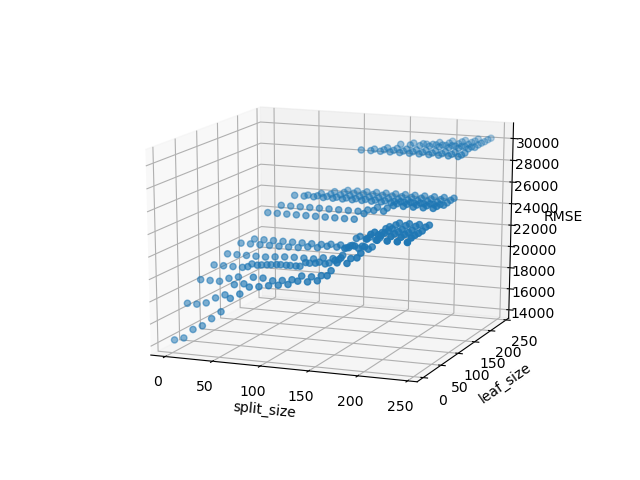
\includegraphics[width=10.6cm]{tree}
        \centering
    \end{figure}

    Utilizzando valori per i parametri di tuning l'errore del sistema è:
    \begin{center}
        \begin{tabular}{|c|c|c|}
            \hline
             & \textbf{RMSE} & \textbf{MAPE} \\
            \hline
            Regression Tree & $24598.45$ &  $9.84\%$ \\
            \hline
        \end{tabular}
    \end{center}


    \subsection{Pruned Regression Tree}
    Attraverso la metodologia del pruning si genera prima un albero molto grande
    (verranno utilizzati i valori $\textit{split\_size}=2$ e $\textit{leaf\_size}=1$),
    per poi generare a partire da questo una serie di subtree sempre più piccoli.
    L'albero creato sul dataset presenta 5575 nodi foglia, successivamente l'
    algoritmo di pruning genera 4377 sottoalberi. I seguenti valori di errore sono stati
    calcolati tramite 5 fold cross valdation e scegliendo per ogni fold il subtree con le 
    prestazioni migliori sul test set.

    \begin{center}
        \begin{tabular}{|c|c|c|}
            \hline
             & \textbf{RMSE} & \textbf{MAPE} \\
            \hline
            Pruned Regression Tree & $16787.71$ &  $3.9\%$ \\
            \hline
        \end{tabular}
    \end{center}


    \subsection{Bagging}
    Per valutare le performance dell'apprendimento tramite Bagging verrà utilizzato
    l'errore sull dataset out of bag, in modo da avere una metrica di errore
    molto simile all'errore in cross validation. Verrà quindi addestrato il sistema
    sull'intero dataset creando \textit{bagging\_size} alberi per la predizione.
    Il valore RMSE al variare di \textit{bagging\_size} è presentato nel seguente
    grafico: 
    \begin{figure}[h]
        \caption{Valori di RMSE diversi al variare di \textit{bagging\_size}
        }
        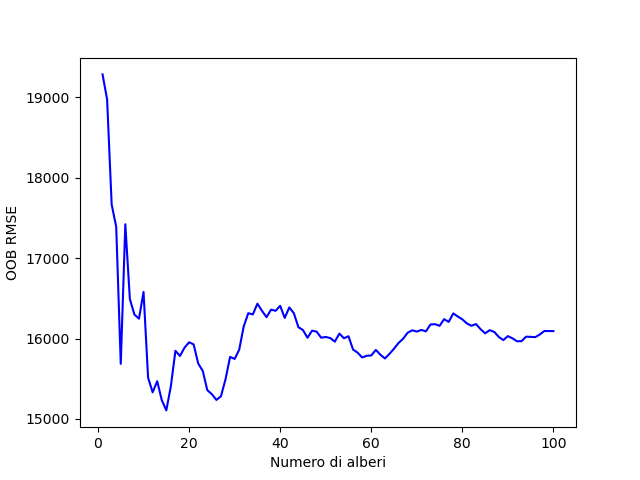
\includegraphics[width=10.6cm]{bag}
        \centering
    \end{figure}



    Verrà scelto il bagging size che fornisce l'OOB Error minore. Per questo dataset 
    il valore scelto è 17, che presenta il seguente errore:


    \begin{center}
        \begin{tabular}{|c|c|c|}
            \hline
             & \textbf{RMSE} & \textbf{MAPE} \\
            \hline
            Bagging  & $15105.90$ &  $8.69\%$ \\
            \hline
        \end{tabular}
    \end{center}

    
    \subsection{Random Forest}
    Per la costruzione della Random Forest verrà utilizzato il valore 25
    per il parametro \textit{bagging\_size} (corrispondente ad uno dei minimi
    locali presenti nel grafico precedente).
    Verrà mostrato come varia l'RMSE al variare del numero di feature 
    considerate per ogni split. I valori considerati saranno (con $p$ numero di feature
    del dataset) $1$, $p/3$, $\sqrt{p}$, $\log_2{(p)}$.

    \begin{figure}[h]
        \caption{Valori di RMSE diversi al variare del numero
        di feature considerate per lo split.
        }
        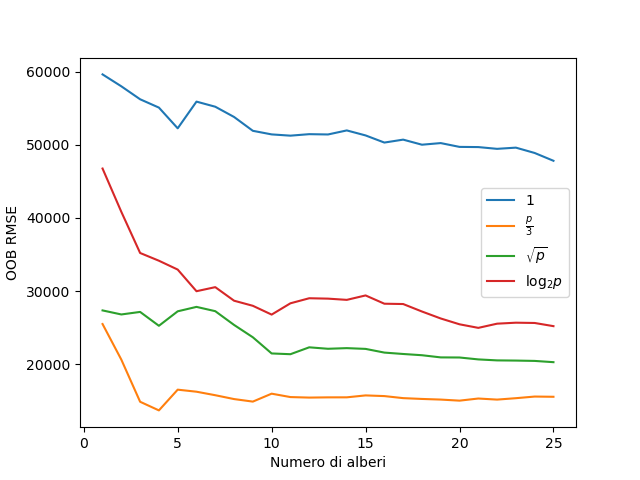
\includegraphics[width=10.6cm]{random}
        \centering
    \end{figure} 


    \begin{center}
        \begin{tabular}{|c|c|c|}
            \hline
            \textbf{Random Forest} & \textbf{RMSE} & \textbf{MAPE} \\
            \hline
            $1$ & $47812.88$ &  $220.98\%$ \\
            $p/3$ & $13715.31$ &  $8.18\%$ \\
            $\sqrt{p}$ & $20303.16$ &  $16.35\%$ \\
            $\log_2{(p)}$ & $24988.88$ &  $38.47\%$ \\
            \hline
        \end{tabular}
    \end{center}

    \subsection{Confronto risultati}
    Dai risultati ottenuti possiamo concludere che la metodologia migliore per il
    dataset scelto è l'utilizzo di alberi di regressione potati, in quanto permettono
    di fornire delle predizioni con un errore assoluto maggiore rispetto a Bagging o Random
    Forest, ma un errore relativo molto più piccolo rispetto alle altre metodologie (permette
    di avere errori piccoli su dati piccoli e errori più grandi su dati grandi). Dal punto
    di vista dell'efficenza il metodo Random Forest risulta il migliore in quanto 
    il considerare una piccola porzione dell feature permette di rendere molto 
    veloce la ricerca di un punto di split ottimale.
    \begin{center}
        \begin{tabular}{|c|c|c|}
            \hline
            \textbf{Sistema} & \textbf{RMSE} & \textbf{MAPE} \\
            \hline
            Regression Tree & $32058.9$ &  $17.60\%$ \\
            Pruned Regression Tree  & $16787.7$ &  $3.9\%$ \\
            Bagging  & $15105.90$ &  $8.69\%$ \\
            Random Forest & $13715.31$ &  $8.18\%$ \\
           
           
            \hline
        \end{tabular}
    \end{center}

    \begin{thebibliography}{9}
        \bibitem{esl} 
        Hastie, T., Tibshirani, R., \& Friedman, J. (2009). 
        The elements of statistical learning: data mining, 
        inference, and prediction. Springer Science \& Business Media.
        
        \bibitem{cart}
        Breiman, L., Friedman, J., Stone, C. J., \& Olshen, R. A. (1984). 
        Classification and regression trees. CRC press.

        \bibitem{norvig}
        Russell, S., \& Norvig, P. 
        (2002). Artificial intelligence: a modern approach.

        \bibitem{pruning}
        Minimal Cost Complexity Pruning (2020)
        \\\texttt{https://online.stat.psu.edu/stat508/lesson/11/11.8/11.8.2}
        
        \bibitem{ai}
        Poole, D. L., \& 
        Mackworth, A. K. (2010). 
        Artificial Intelligence: foundations of
         computational agents. Cambridge University Press.

        
        \bibitem{bias}
        Fortmann-Roe, S. (2012). Understanding the bias-variance tradeoff. 
        \\\texttt{http://scott.fortmann-roe.com/docs/BiasVariance.html} 
        
        \end{thebibliography}









    









    


    


\end{document}